% Generated by extension/semipaired/make_assets.py. Do not edit.
\definecolor{propcol}{HTML}{217D91}
\definecolor{pairedcol}{HTML}{5D6670}
\definecolor{semicol}{HTML}{C9803A}
\definecolor{champcol}{HTML}{8E4B8C}
\definecolor{ridgecol}{HTML}{9AA3AB}
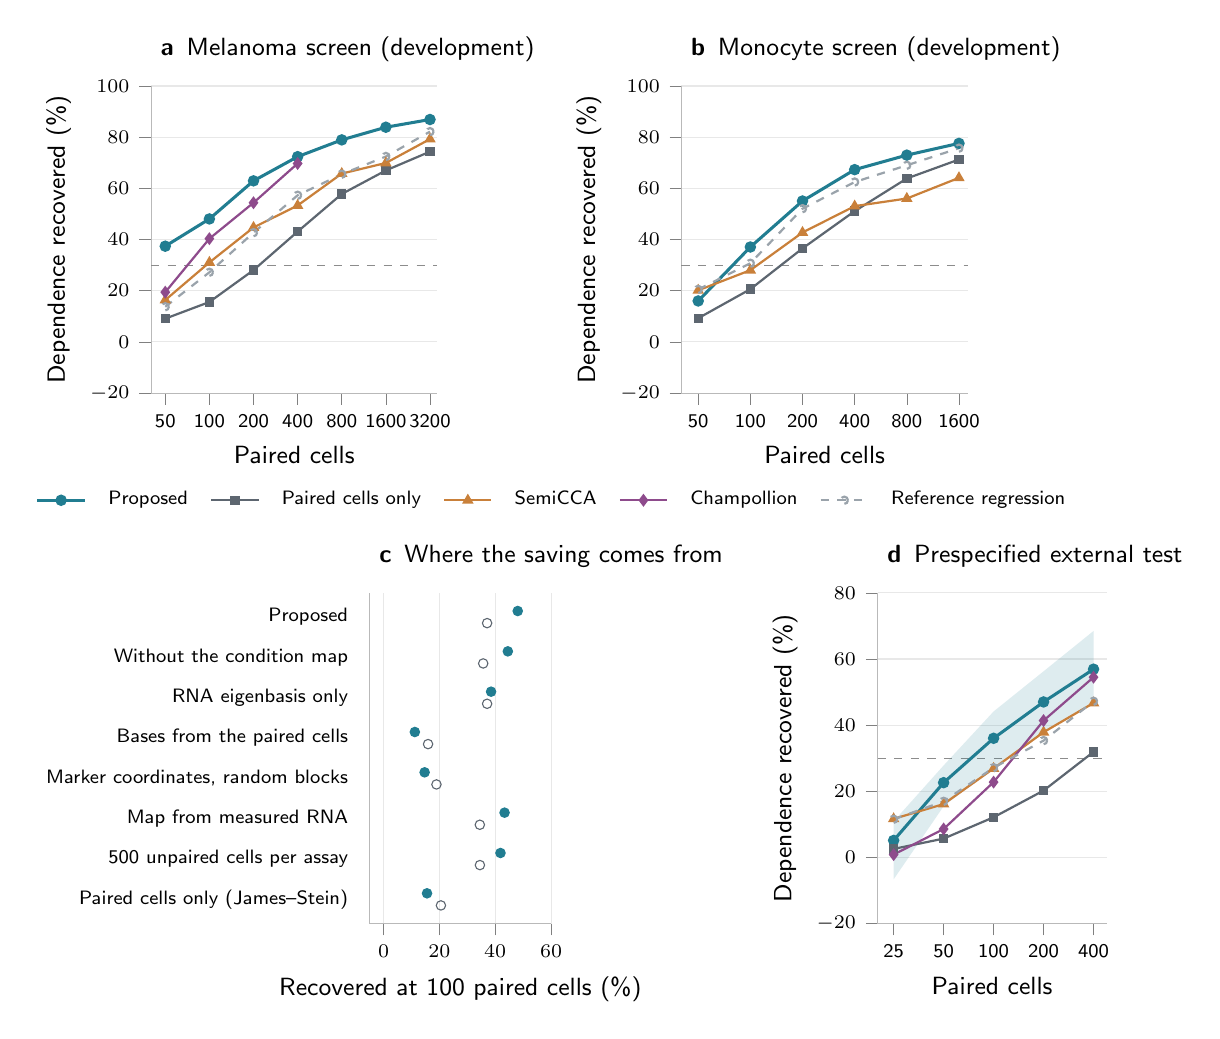
\begin{tikzpicture}[font=\sffamily]
\begin{axis}[name=a,scale only axis,width=.3\textwidth,height=3.9cm,xmode=log,log basis x=2,
 xmin=40,xmax=3600,ymin=-20,ymax=100,xtick={50,100,200,400,800,1600,3200},xticklabels={50,100,200,400,800,1600,3200},ytick={-20,0,20,40,60,80,100},
 xlabel={Paired cells},ylabel={Dependence recovered (\%)},
 title={\textbf{a}\enspace Melanoma screen (development)},
 axis x line*=bottom,axis y line*=left,tick align=outside,ymajorgrids=true,grid style={gray!18},axis line style={gray!55},tick label style={font=\sffamily\scriptsize},label style={font=\sffamily\small},clip=false,title style={font=\sffamily\small,at={(0,1)},anchor=base west,yshift=5pt}]
\draw[dashed,black!45] (axis cs:40,30) -- (axis cs:3600,30);
\addplot[color=propcol,line width=1.1pt,mark=*,mark size=1.5pt] coordinates { (50,37.41) (100,48.06) (200,62.94) (400,72.39) (800,78.95) (1600,83.90) (3200,86.91) };
\addplot[color=pairedcol,line width=.8pt,mark=square*,mark size=1.3pt] coordinates { (50,9.10) (100,15.60) (200,28.06) (400,43.11) (800,57.81) (1600,67.01) (3200,74.36) };
\addplot[color=semicol,line width=.8pt,mark=triangle*,mark size=1.6pt] coordinates { (50,16.36) (100,31.06) (200,44.72) (400,53.32) (800,65.78) (1600,69.93) (3200,79.27) };
\addplot[color=ridgecol,line width=.8pt,dashed,mark=o,mark size=1.3pt] coordinates { (50,13.74) (100,27.21) (200,42.70) (400,57.30) (800,65.54) (1600,72.46) (3200,82.17) };
\addplot[color=champcol,line width=.8pt,mark=diamond*,mark size=1.7pt] coordinates { (50,19.44) (100,40.35) (200,54.39) (400,69.73) };
\end{axis}
\begin{axis}[at={(a.outer north east)},anchor=outer north west,xshift=.3cm,name=b,scale only axis,width=.3\textwidth,height=3.9cm,xmode=log,log basis x=2,
 xmin=40,xmax=1800,ymin=-20,ymax=100,xtick={50,100,200,400,800,1600},xticklabels={50,100,200,400,800,1600},ytick={-20,0,20,40,60,80,100},
 xlabel={Paired cells},ylabel={Dependence recovered (\%)},
 title={\textbf{b}\enspace Monocyte screen (development)},
 axis x line*=bottom,axis y line*=left,tick align=outside,ymajorgrids=true,grid style={gray!18},axis line style={gray!55},tick label style={font=\sffamily\scriptsize},label style={font=\sffamily\small},clip=false,title style={font=\sffamily\small,at={(0,1)},anchor=base west,yshift=5pt}]
\draw[dashed,black!45] (axis cs:40,30) -- (axis cs:1800,30);
\addplot[color=propcol,line width=1.1pt,mark=*,mark size=1.5pt] coordinates { (50,16.01) (100,37.09) (200,55.07) (400,67.32) (800,72.99) (1600,77.59) };
\addplot[color=pairedcol,line width=.8pt,mark=square*,mark size=1.3pt] coordinates { (50,9.26) (100,20.61) (200,36.55) (400,51.11) (800,63.87) (1600,71.28) };
\addplot[color=semicol,line width=.8pt,mark=triangle*,mark size=1.6pt] coordinates { (50,20.16) (100,28.03) (200,42.76) (400,53.06) (800,56.04) (1600,64.12) };
\addplot[color=ridgecol,line width=.8pt,dashed,mark=o,mark size=1.3pt] coordinates { (50,20.51) (100,30.74) (200,52.06) (400,62.48) (800,69.02) (1600,75.71) };
\end{axis}
\path (a.outer south west) -- (b.outer south east) coordinate[pos=.5] (legab);
\begin{axis}[hide axis,scale only axis,width=1pt,height=1pt,xmin=0,xmax=1,ymin=0,ymax=1,at={(legab)},anchor=north,yshift=-2pt,legend style={draw=none,font=\sffamily\scriptsize,at={(0.5,0.5)},anchor=north,legend columns=5,column sep=6pt,cells={anchor=west}}]
\addlegendimage{color=propcol,line width=1.1pt,mark=*,mark size=1.5pt}
\addlegendentry{Proposed}
\addlegendimage{color=pairedcol,line width=.8pt,mark=square*,mark size=1.3pt}
\addlegendentry{Paired cells only}
\addlegendimage{color=semicol,line width=.8pt,mark=triangle*,mark size=1.6pt}
\addlegendentry{SemiCCA}
\addlegendimage{color=champcol,line width=.8pt,mark=diamond*,mark size=1.7pt}
\addlegendentry{Champollion}
\addlegendimage{color=ridgecol,line width=.8pt,dashed,mark=o,mark size=1.3pt}
\addlegendentry{Reference regression}
\end{axis}
\begin{axis}[at={(a.outer south west)},anchor=outer north west,yshift=-.8cm,name=c,scale only axis,width=.19\textwidth,height=4.2cm,xmin=-5,xmax=60,
 ymin=.4,ymax=8.6,ytick={1,2,3,4,5,6,7,8},
 yticklabels={{Paired cells only (James--Stein)},{500 unpaired cells per assay},{Map from measured RNA},{Marker coordinates, random blocks},{Bases from the paired cells},{RNA eigenbasis only},{Without the condition map},{Proposed}},
 xtick={0,20,40,60},xlabel={Recovered at 100 paired cells (\%)},
 title={\textbf{c}\enspace Where the saving comes from},
 axis x line*=bottom,axis y line*=left,tick align=outside,xmajorgrids=true,grid style={gray!18},axis line style={gray!55},tick label style={font=\sffamily\scriptsize},label style={font=\sffamily\small},clip=false,title style={font=\sffamily\small,at={(0,1)},anchor=base west,yshift=5pt},y tick style={draw=none}]
\addplot[only marks,mark=*,mark size=1.7pt,color=propcol] coordinates { (15.56,1.15) (41.88,2.15) (43.34,3.15) (14.70,4.15) (11.19,5.15) (38.51,6.15) (44.51,7.15) (48.06,8.15) };
\addplot[only marks,mark=o,mark size=1.7pt,color=pairedcol] coordinates { (20.54,0.85) (34.51,1.85) (34.48,2.85) (18.94,3.85) (15.93,4.85) (37.09,5.85) (35.69,6.85) (37.09,7.85) };
\end{axis}
\begin{axis}[at={(c.outer north east)},anchor=outer north west,xshift=.4cm,name=d,scale only axis,width=.24\textwidth,height=4.2cm,xmode=log,log basis x=2,
 xmin=20,xmax=480,ymin=-20,ymax=80,xtick={25,50,100,200,400},xticklabels={25,50,100,200,400},ytick={-20,0,20,40,60,80},
 xlabel={Paired cells},ylabel={Dependence recovered (\%)},
 title={\textbf{d}\enspace Prespecified external test},
 axis x line*=bottom,axis y line*=left,tick align=outside,ymajorgrids=true,grid style={gray!18},axis line style={gray!55},tick label style={font=\sffamily\scriptsize},label style={font=\sffamily\small},clip=false,title style={font=\sffamily\small,at={(0,1)},anchor=base west,yshift=5pt}]
\draw[dashed,black!45] (axis cs:20,30) -- (axis cs:480,30);
\fill[propcol,opacity=.15] plot coordinates { (25,-6.62) (50,15.48) (100,27.06) (200,37.85) (400,46.54) (400,68.48) (200,56.28) (100,44.14) (50,27.81) (25,10.92) } -- cycle;
\addplot[color=propcol,line width=1.1pt,mark=*,mark size=1.5pt] coordinates { (25,5.15) (50,22.61) (100,36.03) (200,47.02) (400,56.93) };
\addplot[color=pairedcol,line width=.8pt,mark=square*,mark size=1.3pt] coordinates { (25,2.58) (50,5.70) (100,12.15) (200,20.22) (400,31.92) };
\addplot[color=semicol,line width=.8pt,mark=triangle*,mark size=1.6pt] coordinates { (25,11.67) (50,16.14) (100,26.91) (200,37.87) (400,46.71) };
\addplot[color=champcol,line width=.8pt,mark=diamond*,mark size=1.7pt] coordinates { (25,0.86) (50,8.60) (100,22.78) (200,41.38) (400,54.50) };
\addplot[color=ridgecol,line width=.8pt,dashed,mark=o,mark size=1.3pt] coordinates { (25,11.54) (50,16.97) (100,27.13) (200,35.33) (400,47.22) };
\end{axis}
\end{tikzpicture}
